\chapter{光照估计数据集}
%%一种方法是从single-exposure 估计HDR,也可以用来扩充HDR数据集,但是效果不好。
\section{引言}
对于深度学习任务来说,训练数据的规模、质量对网络最终的表现有着直接的影响。
小规模的数据、低质量的数据、不平衡的数据都可能会导致网络训练失败。
从图片估计光照是一个非常复杂的问题,小规模低质量的数据往往很难训练出较好的预测网络。
目前用于光照估计问题的数据集比较有限,主要包括大规模的低动态范围(LDR)全景图和小规模的高动态范围(HDR)全景图。
这两类数据集都在规模和质量上,无法同时满足训练一个鲁棒的光照估计网络的条件。
因此本文将通过收集、拍摄、筛选、整理等多个严格细致的步骤,构建一个同时包含多类场景的、多种光照条件,而且具有一定规模的光照估计数据集。

本章主要介绍该数据集的构建方式以及在该数据集上的对比试验。本章内容中,首先对低动态范围全景图像和高动态范围全景图像做出介绍;然后阐述HDR全景图的主要拍摄与合成方法;接着展示了用HDR全景图像构建光照估计数据集的若干方法,最后在该数据集上进行多项对比实验,给出了数据集质量和规模对于光照估计问题的影响。

\section{全景图像简介}
全景图(panorama)是一种广角图,可以以画作、照片、影片、三维模型的形式存在。全景图这个词最早由爱尔兰画家罗伯特·巴克提出,用以描述他创作的爱丁堡全景画。现代的全景图多指通过相机拍摄并在计算机上加工而成的图片\cite{wikipedia}。全景图存储了以相机位置为中心的每个角度的颜色信息,颜色信息与普通图片类似,常用RGB三个通道分别存储。全景图根据其中的颜色数值范围,可分为低动态范围全景图和高动态范围全景图。

\subsection{获取}
拍摄全景图像的方式主要有两类。
一类是使用专业的全景相机拍摄设备,这类设备大多由数个鱼眼镜头形式的广角相机组成。
在拍摄时,设备中的相机使用相同的相机参数同时拍摄,随后内置的固件或软件会对所拍摄到的图像进行投影变换、校正、拼接,形成一张全景图。
另外一类是使用普通相机和相机旋转装置,对多个角度拍摄,随后在手动利用拼接算法或拼接软件将这些图像连接到一起。
由于这种方式拍摄到的图片并不在同一个时刻,所以需要保证场景中不能包含过多的快速运动的物体。
此外,大多数的现代智能手机都提供了手动拍摄“全景图”的方式。
不过需要注意的是,由于相机视角范围限制,以人体为轴旋转手机相机拍摄到的“全景图”多称为“宽景图”,
因为顶部视角和底部视角的区域仍然有很大缺失。

\subsection{投影方式}
全景图像的存储需要考虑投影方式和颜色的数值类型。
在全景图像中,以相机为中心的视场可以被视为一个球体的表面,
因此在存储和浏览全景图时,需要将全景球表面投影在二维表面中。
常见的投影方式有等距投影,圆柱投影,球形投影,立方体贴图投影,立体投影等。
\begin{itemize}
\item \textbf{圆柱投影}(cylindrical projection)该投影方式是将全景球置于其外切圆柱内,并由球心向圆柱面做投影,随后将圆柱内表面横向展开后的图像即为球形全景图的圆柱投影。这种投影下的全景图在两极会发生无限的纵向拉伸,因此圆柱投影后的图像无法包含靠近两极的信息,也即这种投影方式无法表示垂直视角为180\degree的全景图。柱面投影是传统摆动镜头全景胶片相机所提供的标准投影方式。相对于全角度的全景图,该投影方式更适合在垂直视角小于120\degree的宽景图,常用于现代智能手机的全景图预览。
\item \textbf{等距投影}(equirectangular projection), 也称等距圆柱投影。该投影方式是将球面的经度和纬度坐标线性变换为图像空间的横纵坐标。经过投影处理后的全景图像是一幅宽高比例为2:1的图片。这种投影的特点是越接近两级,图像的变形就越严重。投影后的全景图在预览时一目了然,而且这种投影方式较为简单,是存储和预览全景图最常见的方式之一。
\item \textbf{圆周鱼眼投影}(circumferential fisheye projection),也称圆形投影或镜面球投影,为角投影的一种。这样的投影图像看起来像一个用超级圆形鱼眼镜头所拍摄的图片,虽然这种投影方式依然覆盖360\degree的视角,但是其边缘却被极端扭曲和变形。这种投影方式常见于全景图拍摄设备中。全景相机一般由两个朝向相反的180\degree视角鱼眼镜头。每个镜头所拍摄到的图片均为一个垂直和水平视角各180\degree的圆周鱼眼投影视图。
\item \textbf{立方体贴图投影}(cubemap projection)在计算机图形学中,立方体投影是常用的环境映射方法之一,常用于游戏场景中的天空盒,相当于等距柱状投影的优化版,环境投影到立方体之后可分六个正方形纹理来存储;或者将立方体展开,存储于一个纹理中的六个区域内。 
在全景图像及视频中,立方体投影将球形视频映射到它的外接立方体上,立方体的上下两个面分别对应两极区域,中间的四个面对应赤道区域。
\item \textbf{立体投影} (stereographic projection),即常见的小行星投影方式。
\end{itemize}
\begin{figure}[!htbp]
    \centering
    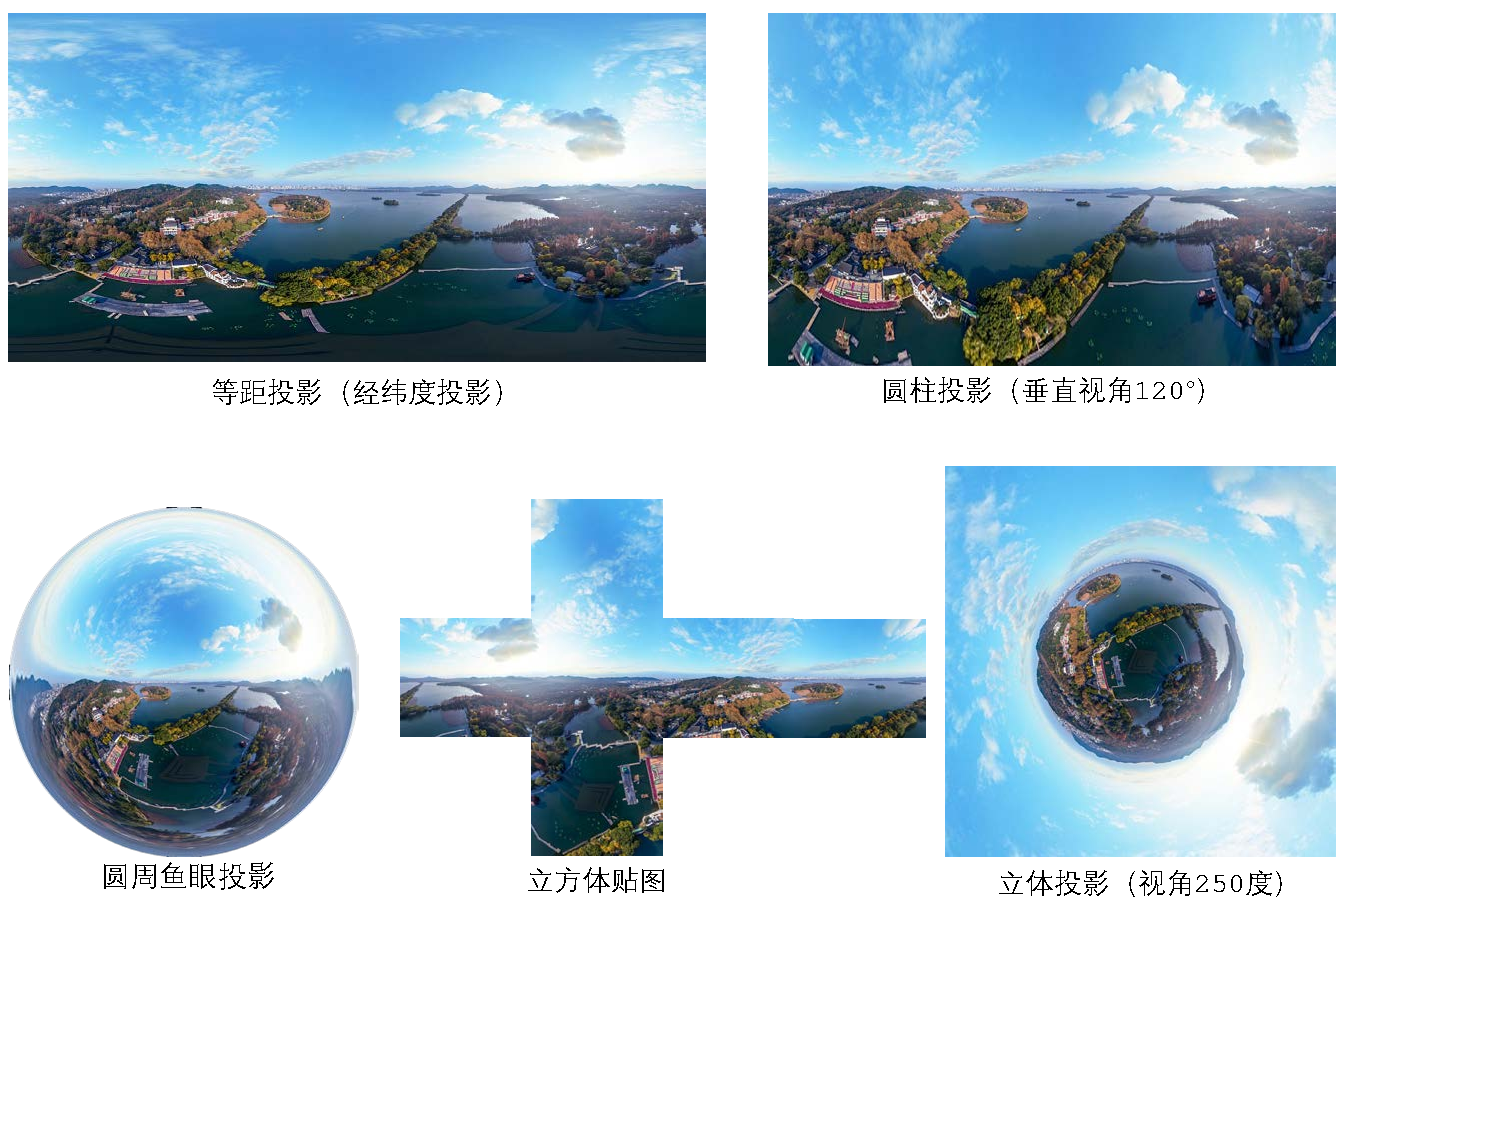
\includegraphics[width=1.0\textwidth]{Img/panorama-projection.pdf}

    \caption[全景图的几种投影方式]
    {
        \label{fig:panorama-projection}
        全景图几种投影方式。等距投影是常见的全景图投影方式,包括了所有视角的信息。圆柱投影的特点致使它不可能有180\doge的垂直视角;圆周鱼眼投影可以显示出所有视角的信息,但是从中可以看到,靠近圆形边缘的区域被极度扭曲,这会因为计算误差导致精度的损失;立方体贴图是计算机图形学中常用的投影方式;立体投影方式看起来像一颗星球,因此也被成为小行星投影方式,这种方式也无法展示所有视角的信息。
    }
\end{figure}
除此之外,还有墨卡托投影、正弦投影等、直线投影用于不同的领域。图\ref{fig:panorama-projection}展示了几种常见的投影方式。

\subsection{动态范围}
图像的动态范围(dynamic Range)是指一个图像中最亮和最暗部分之间的相对比值。\cite{wikipedia}。
根据动态范围的大小可以将图像分为低动态范围(或称为标准动态范围)图像和高动态范围图像。
传统的8位图像将颜色值存储为[0, 255]范围内的整数,低动态范围图像中的颜色只能在这256个数中取值。图\todo{图片}展示了同一场景不同曝光条件下的照片,可以看出每幅图片都有一定的过曝和欠曝区域。例如在过曝图片中,太阳和其周围区域的颜色均为白色,但实际上太阳的亮度要远远高过天空的亮度;同样的,在欠曝区域中,虽然大部分区域同为黑色,但实际上这些区域的明暗程度也是千差万别的。

而相比低动态范围的图像,高动态范围图像可以提供更多的动态范围(理论上是0到无限大)。高动态范围全景图也是具有这种动态范围的全景图像。高动态范围全景图的动态范围可以高达$2^{32}$,而人类的眼睛所能看到的范围是$10^5$左右\cite{wikipedia}。因此高动态范围全景图像可以作为真实的光照信息,这是低动态范围全景图不能比拟的。
\todo{图片}展示了两组使用低动态范围全景图和高动态范围全景图的渲染结果,可以看出,使用低动态范围全景图渲染的结果颜色值对比平缓,看起来很不真实。而使用高动态范围全景图作为光照时,渲染结果包含了足够的对比度和锐利的阴影。\todo{图片}中的第二组使用了包含更亮光源的场景作为对比,它们之间的差异更加明显。
为方便叙述和浏览,下文中的LDR将代指低动态范围全景图,HDR将代指高动态范围全景图。
%% page 1
\subsection{HDR的获取与存储}
HDR全景图的获取方式与普通全景图类似,不过由于HDR包含了更大的动态范围。而普通相机单词拍摄无法满足这个要求,因此需要使用对每个视角的图像都要使用不同的曝光值来进行拍摄。
HDR全景图的获取分为多曝光拍摄,多视角拍摄,全景图拼接,清洗和筛选,曝光融合五个步骤。
\begin{itemize}
    \item \textbf{多曝光拍摄}。HDR图像通常无法直接由拍摄设备直接获取,因此需要利用不同的曝光值对同一场景多次拍摄。曝光值通常由相机的ISO、快门速度、光圈大小共同决定。图\todo{图片}展示了在不同曝光条件下拍摄的图像。
    \item \textbf{多视角拍摄}。单个相机的视角有限,在合成全景图之前,需要对场景的不同视角拍摄。为了保证拼接后的图片质量,拍摄时相机的镜头不能有太大的平移。因此拍摄全景图时,相机位置多由精密的机械装置自动控制。图\todo{图片}展示了一个用于拍摄全景图的机械装置。此外需要注意的是,对于每个拍摄视角,拍摄时的曝光值序列和相机的其它参数(例如白平衡,相机视场范围等)要完全一致,以保证在全景图拼接时的各个视角图片的一致性。
    \item \textbf{全景图拼接}。使用普通相机对多个视角进行拍摄后,需要将这些图片拼接到一起。这通常需要做图片间的特征匹配等等,目前全景图的拼接有较为成熟的算法和工具,这里不再展开叙述。另外,目前市面上出现了一种专门用于拍摄全景图的全景相机,其中有些全景相机支持通过调节ISO,快门速度等拍摄多种曝光条件下的全景图,例如小米全景相机\cite{xiaomi}等。使用这种相机可以省去图像拼接的步骤,每次拍摄只需要关注相机的曝光即可,也可以避免拼接时产生的瑕疵结果。图\todo{图片}展示了使用全景相机拍摄全景图的方式之一。
    \item \textbf{清洗和筛选}。拍摄结果中不可避免的会有一些质量较差的图片,因此需要进行筛除和清理。质量较差的图片通常包括:图片中场景不一致(经常由移动物体在不同时刻被拍摄导致)、图片色差过大、图片噪点过多(经常由较暗场景中使用过大的ISO导致)、相机本身的拍摄异常等。这些都需要人工观察、筛选、清理和重拍,以保证最终合成的HDR全景图的质量。
    \item \textbf{曝光HDR融合}。当获得多张不同曝光的全景图后需要将他们融合为一张HDR图,常见的融合算法有基于基于信息熵的算法、基于双边滤波的算法、基于亮度梯度大小的算法、基于拉普拉斯金字塔的算法等。曝光融合工具中,PTGUI\cite{ptgui}能够提供很好的融合结果。
\end{itemize}
曝光融合后的全景图就是一幅HDR全景图,这种全景图包含了很高的动态范围,可以作为场景真实光照的表示。HDR全景图像的投影方式和普通全景图完全一致,它们之间的区别只是每个像素位置的数值类型和数值范围不同,常见的HDR图像保存格式有TIFF, HDR, RGBE, EXR等。

\section{构建HDR全景数据集}
本节主要介绍构建HDR全景数据集的方法与步骤。构建时需要考虑数据的多样性,保证数据质量。
\subsection{场景选择}
HDR全景数据集需要考虑到场景的多样性,为此,本文选取了多个场景进行拍摄,包含了室内、室外,森林,公园,公寓,小区,建筑群等多种常见场景,晴天,阴天,多云等多种气象条件,清晨、中午、下午、傍晚、夜间等多种拍摄时间,以及春夏秋冬四季多个拍摄季节,其中各场景比例如表格\todo{表格}所示。
\subsection{拍摄设备选择}
拍摄HDR全景图的方式有两种,一种是使用普通相机多次拍摄并进行拼接,另一种是直接使用全景相机拍摄,本文采用的的方式是后者,即直接使用全景相机拍摄,这样可以避免大量的拼接操作,只需要根据场景调整不同的曝光范围即可。
\subsection{曝光融合工具}
在进行曝光融合时,通过多种曝光融合工具的对比,发现PTGUI\cite{ptgui}能够提供很好的融合结果,因此本文在构建该光照估计数据集时主要使用此工具进行曝光融合,融合时的参数如表格\todo{表格}所示。

通过如上步骤,我们共拍摄了约5000张全景图像,经过清理和筛选,共合成了约550组HDR全景图。图\todo{图片}是展示了部分HDR全景图,可以看出该数据集包含了多种场景和光照条件,而且图片质量较高,几乎没有早点和拼接痕迹。
\section{构建光照估计数据集}
\section{数据集对光照估计效果的影响分析}
为了验证数据集在光照估计中的有效性,本文设计另一个基础的光照估计深度学习网络。并在该网络上使用多种数据集进行训练和测试,
\subsection{用于对比的光照估计网络}
从图片预测整个HDR图往往比较困难,为了有效地在该数据集上进行试验,本文搭建了一个从图片到球形谐波系数的网络。
\subsection{数据集划分}
对比试验主要分为三个部分,首先是对比不同的数据规模对光照估计网络的影响,其次是对比数据的多样性大小对光照估计网络的影响,最后是本文构建的数据集和部分已有数据集的对比。
在前两部分实验中,所有的数据均为本文所构建的数据集,因此将该数据集按照训练集400、测试集100、验证集50的比例划分后,在训练集上训练,以验证集上的结果作为实验结果进行分析对比和验证。
在与其它数据集对比的实验中,为了公平实验,用作对比和分析的数据均由真实的图片和对应的HDR全景图作为对比,而本文所构建的数据均用于训练光照估计网络。
此外,在数据划分时,是在HDR全景数据上进行划分后,再在每一幅HDR全景图中提取视角图片,而不是在提取的图片中进行划分,这样可以保证同一幅HDR全景图不会同时出现再不同的数据集中。
\subsection{数据的规模对光照估计的影响}
\subsection{数据多样性对光照估计的影响}
\subsection{与其它数据集的对比}
本文与其它数据集在两个方面进行对比,一个是
\section{讨论}
%% 优点
可以看出,HDR全景图的拍摄需要对同一场景多次拍摄,因此快速变动的场景。不过对于光照估计问题来说,该数据集的多样性已经足够
%% 不足
规模依然可以扩充,地点可以增多,动态范围可以继续增加。
\section{本章小结}